
\section{Electronics - Ali Mokdad}
The electronics department constitutes a link between programming and mechanical structure, by establishing the movement of the mechanical parts of the Butler with respect to the code. This section declares the electronic components used in the Butler project including the motors, motor controllers and development boards.

\subsection{Motors and gearboxes - Ali Mokdad}  \label{MotorsNGearboxes}


\subsubsection{Requirements}
The actuators of the Butler have been chosen with respect to mechanical calculations based on the weight of the Butler arm to choose the correct motors according to two main parameters: Torque and speed. The calculations have been divided in two parts: The first part is concerning the different parts of the arm of the Butler, and the second part is concerning the base of the Butler. 

\begin{enumerate}
\item \textbf{Calculations for the arm:}\\
The arm of the Butler is connected to the base from the shoulder part, where a metal plate holding the motors M1 and M2 constitutes the link between the arm and the base of the Butler.
The arm of the Butler consists of three parts: A shoulder joint rotated by M1 arm, an elbow joint rotated by M2 arm and a wrist rotated by M3 arm. Note that M2 arm is located next to M1 arm in order to make the arm lighter. Figure~\ref{fig:Arm structure of the Butler}  represents the weight distribution considered for the arm:

\begin{figure}[h!]
\centering
\captionsetup{justification=centering}
\includegraphics[width=1\textwidth]{Electronics/arm.jpg}
\caption{Arm structure of the Butler where M2 arm is located next to M1 arm in order to make the arm lighter}
\label{fig:Arm structure of the Butler}
\end{figure}


The maximum mass of the whole arm  is:

\begin{equation} \label{eq:m_total}
\begin{split}
M_{total} & = m1 + m2 + m3\\
& = 0.5 + 0.3 + 1\\
& = 1.8 Kg\\
\end{split}
\end{equation}

In order to calculate the torque needed for each motor, the centre of mass of the parts needed to be lifted by each of the motors needs to be calculated, by taking the position of each motor as the origin (when X=0).
The Centre of mass is calculated by the following equation:

\begin{equation} \label{eq: X_cm}
\begin{split}
X_{cm} & = \frac{m_1*X_1 + m_2*X_2 + m_3*X_3}{m_1 + m_2 + m_3} \\ 
\end{split}
\end{equation}
Where X1, X2 and X3 are the distances from the motor position (origin) to the centre of gravity of each part of the arm.\\

\begin{itemize}

\item \textbf{For M1 arm}: 
\begin{equation} \label{eq: X_Cm1}
\begin{split}
X_{Cm1} & = \frac{(0.15*0.5) + (0.4*0.3) + (0.6*1)}{0.5 + 0.3 +1} \\
& = 0.44
\end{split}
\end{equation}


 
The torque needed from M1 arm is:
\begin{equation} \label{eq: T_M1}
\begin{split}
T_{NeededM1} & = X_{Cm1} *  M_{total} * gravity\\
& = 0.44 * 1.8 * 9.82\\
& = 7.8 Nm\\
\end{split}
\end{equation}

\item \textbf{For M2 arm:} \\
The center of mass needed for M2 arm is:
\begin{equation} \label{eq: X_Cm2}
\begin{split}
X_{Cm2} & = \frac{(0.4*0.3) + (0.2*1) }{0.3 + 1}  \\
& = 0.246
\end{split}
\end{equation}

The torque needed from M2 arm is:
\begin{equation} \label{eq: T_M2}
\begin{split}
T_{NeededM2} & = X_{Cm2}*  M_{afterElbow} * gravity\\
& = 0.246 * (0.3+1) * 9.82\\
& = 3.13 Nm\\
\end{split}
\end{equation}

\item \textbf{For M3 arm:} \\
The center of mass needed for M3 arm is:
\begin{equation} \label{eq: X_Cm3}
\begin{split}
X_{Cm3} & = \frac{(0.1*1)}{1} \\
&= 0.1
\end{split}
\end{equation}

The torque needed from M3 arm is:
\begin{equation} \label{eq: T_M3}
\begin{split}
T_{NeededM3} & = X_{Cm3} *  M_{afterWrist} * gravity\\
& = 0.1 * 1 * 9.82\\
& = 0.982 Nm\\
\end{split}
\end{equation}

\end{itemize}

\item \textbf{Calculations for the base}:\\
The base of the butler consists of two motors: M4 base and M5 base. The motor M4 base is responsible of moving the whole arm of the butler up and down, by rotating a screw attached to a spindle, enabling the arm to move over the axis which is in this case the spindle. The motor M5 base is responsible of making the base of the butler rotate, resulting in a change of the direction.\\

\textbf{For M4 base:}
The selection of the motor M4 base has been fully referred to mechanical requirements based on two major factors: the force produced by the weight of the arm over the motor, and the lead of the spindle attached to a screw. According to calculations made in the mechanics section, the major requirement of the motor M4 base is the speed. The needed speed is 50 Rpm as a minimum with a torque of 0.2 Nm to 0.3 Nm as maximum.
\\

\textbf{For M5 base}
The motor M5 base requires low torque and low speed, in order to rotate the base of the Butler.

\end{enumerate}
In order to make the Butler as efficient as possible, the followings assumptions have been made:
\begin{itemize}
    \item The motors M1 arm, M2 arm, M5 base should be stepper motors since high precision and high torque is required respectively in rotating the whole arm, rotating the elbow joint and rotating the base of the Butler.
    \item The motor M3 arm should be a servo motor, since servos provide extreme precision (but lower torque than stepper motors).
    \item The motor M4 base should be a DC motor since high speed is needed, to be able to rotate the screw fast enough to reach the requirement of 50 RPM as speed of the motor.
\end{itemize}





%%%%%%%%%%%%%%%%%%%%%%%%%%%%%%%%%%%%%%%%%%%%%%%%%%%%%%%%%%%%%%%%%%%%%%%%%%%%%%%%%%%%%%%%%%%%%

\subsubsection{Motors and gearboxes selection}
In order to achieve the motor requirements, the following motors and gear boxes have been chosen:
\\
\begin{enumerate}
    \item \textbf{M1 arm: Rotating the the whole arm of the Butler:}\\\\
    \textbf{Motor:}
    \begin{itemize}
        \item Name: planetary gear unipolar stepper motor\cite{m1}.
        \item Nominal voltage: 9.6 V.
        \item Current: 0.4 A.
        \item Nominal torque: 0.086 Nm.\\
    \end{itemize}
    
    \textbf{Gearbox:}
    \begin{itemize}
        \item Gearbox type: Planetary.
        \item Reduction ratio: 104:1.
        \item Backlash at no-load: less than 1.5 degrees.\\
    \end{itemize}
    
    \textbf{Motor with gearbox:}
    \begin{itemize}
        \item Name: planetary gear unipolar stepper motor.
        \item Weight: 740 g.
        \item Price: 440.46 SEK.
        \item Part number: RB-Dyd-02.
        \item Supplier: Robotshop.
     \end{itemize}
    In order to know if the motor M1 arm combined with the gearbox will be able to carry the weight of the arm, the maximum output torque needs to be calculated. 
    From the specifications above of the motor M1 arm, the maximum output torque is:\\
    \begin{equation} \label{eq: T_M1arm}
    \begin{split}
    T_{M1arm} & = T_{Motor} * R_{max}\\
    & =  0.086 * 104\\
    & = 8.944 Nm\\
    \end{split}
    \end{equation}
    Where T\textsubscript{M1arm} is the maximum output torque of the motor M1 arm, T\textsubscript{Motor} is the nominal torque of the motor without the gearbox, and R\textsubscript{max} the reduction ratio from the gearbox.
    
    In addition, a mechanical gear attached to the motor could modify the final values. The mechanical gear having a reduction ratio of 1:1 for this motor remains the same as the following calculations show:
    \begin{equation} \label{eq: T_M1Final}
    \begin{split}
    T_{M1Final} & = T_{M1arm} * R_{mechanical}\\
    & =  8.944 * 1\\
    & = 8.944 Nm\\
    \end{split}
    \end{equation}
    
    Where T\textsubscript{M1Final} is the final output torque after mechanical gearing, T\textsubscript{M1arm} is the output torque of M1 arm, and R\textsubscript{mechanical} is the reduction ratio of the mechanical gear.
    
    The above combination shows that the output torque of M1 arm (8.944 Nm) exceeds the required torque (7.8 Nm), making the motor chosen sufficient for rotating the arm of the Butler.\\
   
%%%%%%%%%%%%%%%%%%%%%%%%%%%%%%%%%%%%%%%%%%%%%%%%%%%%%%%%%%%%%%%%%%%%%%%%%%%%%%%%%%%%%%%%%%%%%%%%%%%%%%%%%%
    \item \textbf {M2 arm: Rotating the the elbow of the Butler:}\\
    \textbf{Motor:}
    \begin{itemize}
        \item Name: NEMA-17 bipolar stepper motor\cite{M2andM5}.
        \item Nominal voltage: 12 V.
        \item Current: 1.7 A.
        \item Nominal torque: 0.047 Nm\\
       
    \end{itemize}
    
    \textbf{Gearbox:}
    \begin{itemize}
        \item Gearbox type: Planetary.
        \item Reduction ratio: 99.5:1.
        \item Backlash error: 1.5 degrees.\\
    \end{itemize}
    
     \textbf{Motor with gearbox:}
    \begin{itemize}
        \item Name: NEMA-17 bipolar stepper motor with planetary gearbox.
        \item Weight: 564 g.
        \item Price: 801.60 SEK.
        \item Part number: RB-Phi-267.
        \item Supplier: Robotshop.
    \end{itemize}
    
     From the specifications above of the motor M2 arm, the maximum output torque is:\\
    \begin{equation} \label{eq: T_M2arm}
    \begin{split}
    T_{M2arm} & = T_{Motor} * R_{max}\\
    & =  0.047 * 100\\
    & = 4.7 Nm\\
    \end{split}
    \end{equation}
    
    A mechanical gear having a reduction ratio of 2:1 attached to M2 arm modifies the output torque value, as shown below:
    
    \begin{equation} \label{eq: T_M2Final}
    \begin{split}
    T_{M2Final} & = T_{M2arm} * R_{mechanical}\\
    & = 4.7 * 2\\
    & = 9.4 Nm\\
    \end{split}
    \end{equation}
    
    Since the final output torque of M2 arm (9.4 Nm) is higher than the required torque (3.13 Nm), the motor is assumed to be sufficient for rotating the elbow of the Butler.\\
    
%%%%%%%%%%%%%%%%%%%%%%%%%%%%%%%%%%%%%%%%%%%%%%%%%%%%%%%%%%%%%%%%%%%%%%%%%%%%%%%%%%%%%%%%%%%%%%%%%%%%%%%    
    \item \textbf {M3 arm: Rotating the wrist of Butler:}\\\\
   \textbf{Motor:}
    \begin{itemize}
        \item Name: AX18-a dynamixel servo motor\cite{servo}.
        \item Operating voltage: 9 to 12 V.
        \item Current: 2.2 A.
        \item Nominal torque:0.007 Nm.\\
    \end{itemize}
    
    \textbf{Gearbox:}
    \begin{itemize}
        \item Gear built in with the motor.
        \item Gear ratio: 254:1.\\
    \end{itemize}
    
    \textbf{Motor with gearbox:}
    \begin{itemize}
        \item Name: AX18-a dynamixel servo motor.
        \item Weight: 54.5 g.
        \item Price: 792.42 SEK.
        \item Part number:RB-Rbs-101
        \item Supplier: Robotshop. 
    \end{itemize}
    
    According to the specifications above of the motor M3 arm, the maximum output torque is:\\
    \begin{equation} \label{eq: T_M3arm }
    \begin{split}
    T_{M3arm} & = T_{Motor} * R_{max}\\
    & =  0.007 * 254\\
    & = 1.77 Nm\\
    \end{split}
    \end{equation}
    The output torque of M3 arm (1.77 Nm) is higher than the required torque (0.982 Nm), which means that the motor chosen is sufficient. This motor is not attached to a mechanical gear so the output remains the same.\\
    
    
%%%%%%%%%%%%%%%%%%%%%%%%%%%%%%%%%%%%%%%%%%%%%%%%%%%%%%%%%%%%%%%%%%%%%%%%%%%%%%%%%%%%%%%%%%%%%%%%%%%%%%%


    \item \begin{itemize}
        \item  \textbf {M4 base: Rotating a screw attached to a spindle to move all the arm of the Butler:}\\\\
   \textbf{Motor:}
    \begin{itemize}
        \item Name:  Lynxmotion brushed DC gear motor\cite{M4}.
        \item Nominal voltage: 12 V.
        \item Current: 250 mA.
        \item Nominal torque: 0.034 Nm.\\
    \end{itemize}
    
    \textbf{Gearbox:}
    \begin{itemize}
        \item Gear Ratio: 5.2:1.\\
    \end{itemize}
    
    \textbf{Motor with gearbox:}
    \begin{itemize}
        \item Name: Lynxmotion brushed DC gear motor.
        \item Weight: 533 g.
        \item Price: 714.04 SEK.
        \item Part number: RB-Wtc-02.
        \item Supplier: Robotshop.\\
    \end{itemize}
    
    The specifications above result in the following maximum output torque:
    \begin{equation} \label{eq: T_M4base}
    \begin{split}
    T_{M4base} & = T_{Motor} * R_{max}\\
    & =  0.034 * 5.2\\
    & = 0.1768 Nm\\
    \end{split}
    \end{equation}
    
    The output torque obtained (0.1768) compared to the required torque (0.2 to 0.3 Nm) is not enough; But the use of a mechanical gear having a reduction ratio of 50:12 made the values approved, the motor M4 base attached to the mechanical gear resulted in an output torque of:
    \begin{equation} \label{eq: T_M4Final}
    \begin{split} 
    T_{M4Final} & = T_{M4base} * R_{mechanical}\\
    & =  0.1768 * 4.166\\
    & = 0.73 Nm\\
    \end{split}
    \end{equation}
    
    
    The output speed of the motor M4 base is:
    
    \begin{equation} \label{eq: Speed_M4base}
    \begin{split}
    Speed_{M4base} & = speed_{Motor} / R_{max}\\
    & =  2496 / 5.2\\
    & = 480 Rpm\\
    \end{split}
    \end{equation}
    
    The output speed of the motor attached to the mechanical gear is:
    
    \begin{equation} \label{eq: Speed_M4Final}
    \begin{split} 
    Speed_{M4Final} & = Speed_{M4base} / R_{mechanical}\\
    & =  480 / 4.166\\
    & = 115.21 Nm\\
    \end{split}
    \end{equation}
    
    The final output speed obtained (115.21 Rpm) exceeds the demanded speed (50 Rpm), making the motor M4 base chosen approved.\\
    
    \item \textbf{Encoder: Hall effect encoder YC2010}\\
    In order to detect the position and the speed of the motor M4 base, an encoder is required. A \textbf{hall effect encoder YC2010} attached to the motor M4 base gives feedback about the motor position by detecting a change in voltage by magnetic deflection of electrons. The encoder consists of a 2 channel output A and B that are 90 electrical degrees out of phase, which enables direction sensing. The YC2010 encoder consists of the following wires:
    \begin{itemize}
        \item \textbf{Red wire:} Powering up the motor (+).
        \item \textbf{Black wire:} Powering up the motor (-).
        \item \textbf{Green wire:} Hall sensor GND.
        \item \textbf{Blue wire:} Hall sensor VCC.
        \item \textbf{Yellow wire:} Hall sensor channel A Vout.
        \item \textbf{White wire:} Hall sensor channel B Vout.\\
    \end{itemize}
   
    
    \end{itemize}
    
%%%%%%%%%%%%%%%%%%%%%%%%%%%%%%%%%%%%%%%%%%%%%%%%%%%%%%%%%%%%%%%%%%%%%%%%%%%%%%%%%%%%%%%%%%%%%%%%%%%%%%%   
    \item \textbf {M5 base: Rotating the base of the Butler:}\\\\
     \textbf{Motor:}
    \begin{itemize}
        \item Name: NEMA-17 bipolar stepper motor with planetary gearbox\cite{M2andM5}.
        \item Nominal voltage: 12 V.
        \item Current: 1.7 A.
        \item Nominal torque: 0.047 Nm.\\
    \end{itemize}
    
    \textbf{Gearbox:}
    \begin{itemize}
        \item Gearbox type: Planetary.
        \item Reduction ratio: 99.5:1.
        \item Backlash error: 1.5 degrees.\\
    \end{itemize}
    
    \textbf{Motor with gearbox:}
    \begin{itemize}
        \item Name: NEMA-17 bipolar stepper motor with planetary gearbox.
        \item Weight: 564 g.
        \item Price: 801.60 SEK.
        \item Part number: RB-Phi-267.
        \item Supplier: Robotshop.\\
    \end{itemize}
    
    This motor has been chosen after considering that the weight of the Butler will not be held by this motor, in fact the weight will be held by the base platform (i will reference this). 
    This motor has been chosen because of the lack of time, which made choosing an already available motor a must, since the shipping needs time. This motor has the following output torque:
    
    \begin{equation} \label{eq: T_M5base}
    \begin{split}
    T_{M5base} & = T_{Motor} * R_{max}\\
    & =  0.047 * 100\\
    & = 4.7 Nm\\
    \end{split}
    \end{equation}
    
    A mechanical gear having a reduction ratio of 80:20 attached to M5 base modifies the output torque value, as shown below:
    
    \begin{equation} \label{eq: T_M5Final}
    \begin{split}
    T_{M5Final} & = T_{M5base} * R_{mechanical}\\
    & = 4.7 * 4\\
    & = 18.8 Nm\\
    \end{split}
    \end{equation}
\end{enumerate}


%%%%%%%%%%%%%%%%%%%%%%%%%%%%%%%%%%%%%%%%%%%%%%%%%%%%%%%%%%%%%%%%%%%%%%%%%%%%%%%%%%%%%%%%%%%%%

\subsubsection{Price and weight}
The sum of the price and weight for all the motors with the gearboxes are listed below:\\\\
\textbf{Price:} 3550.12 SEK.\\\\
\textbf{Weight:} 2455.5 grams. 

\subsubsection{Conclusion}
The motors chosen for the Butler showed good performance. However, their performance did not reach the expectations desired, where data-sheet values were not fully reached like the torque and speed for example, due to their low cost.
As future work, the motors would be replaced by Maxon Motors, in case of high budget availability, where detailed selection of motor with compatible gearbox and encoder is available with fully explained data-sheets.
%%%%%%%%%%%%%%%%%%%%%%%%%%%%%%%%%%%%%%%%%%%%%%%%%%%%%%%%%%%%%%%%%%%%%%%%%%%%%%%%%%%%%%%%%%%%%%%%%%%%%%%%%%%%%%%%%%%%%%%%%%%%%%%%%%%%%%%%%%%%%%%%%%%%%%%%%%%%%%%%%%%%%%%%%%%%%%%%%%%%%%%%%%%%%%%%%%%%%%%%%%%%%%%%%%%%%%%%%%%%%%%%%%%%%%%%%%%%%%%%%%%%%%%%%%%%%%%%%%%%%%%%%%%%%%%%%%%%%%%

\subsection{Motor controllers - Ali Mokdad}
\label{MotorController}%Do not remove please.
% \subsubsection{Introduction}
In order to control the motors, a motor controller needs to be used. A motor controller enables modifying the speed and the direction of rotation of the motor. Basically, every motor needs a controller to be able to control its performance as desired by the user.

%%%%%%%%%%%%%%%%%%%%%%%%%%%%%%%%%%%%%%%%%%%%%%%%%%%%%%%%%%%%%%%%%%%%%%%%%%%%%%%%%%%%%%%%%%%%%

\subsubsection{Requirements}
The motor controllers for the Butler were chosen with respect to the motor selection process. There are two major types of motor controllers: Stepper motor controller and DC motor controller. For the Butler, since the chosen motors are three stepper motors and one DC motor, then there should be three stepper motor controllers (for the motors M1 arm, M2 arm and M5 base) and one DC motor controller (for the motor M4 base).\\
In addition, the motor controllers should be able to handle the current needed by each motor. For the Butler, two \textbf{stepper} motor controllers should handle 1.7 Amps, and one last stepper motor controller should handle 0.9 Amps. The \textbf{DC} motor controller should handle 0.25 Amps.
%%%%%%%%%%%%%%%%%%%%%%%%%%%%%%%%%%%%%%%%%%%%%%%%%%%%%%%%%%%%%%%%%%%%%%%%%%%%%%%%%%%%%%%%%%%%%
\subsubsection{Motor controllers selection}

In order to fulfill the requirements, the selected motor controllers are: a TB6600\cite{Gpu2017} stepper motor driver and an MD30C\cite{ppp} DC motor driver. Three of the TB6600 stepper motor driver have been used for controlling the three stepper motors M1 arm, M2 arm and M5 base, and one MD30C DC motor driver for controlling the DC motor M4 base.\\
The TB6600 stepper motor driver replaced a Cytron SD02C\cite{123} stepper motor driver tested in the early stages of the project since this SD02C driver resulted in bad performance proving that it is not suitable for driving the selected motors. The conclusion section below states further explanation about the reason why the SD02C stepper motor driver has been replaced by the TB6600 stepper motor drive.

%%%%%%%%%%%%%%%%%%%%%%%%%%%%%%%%%%%%%%%%%%%%%%%%%%%%%%%%%%%%%%%%%%%%%%%%%%%%%%%%%%%%%%%%%%%%%

\subsubsection{Testing motor controllers}
For testing the motor controllers, the following connections needs to be established as shown in figure~\ref{Motor controller connection for testing}.
\begin{itemize}
    \item Connection for powering up the motor controller.
    \item Connection to the motor.
    \item Connection for a PWM signal.
    \item Connection for the direction of rotation.
\end{itemize}

\begin{figure}[h!]
\centering
\includegraphics[width=0.8\textwidth]{Electronics/controller.png}
\caption{Motor controller connection for testing}
\label{Motor controller connection for testing}
\end{figure}%% ALI CHECK CHAT



%%%%%%%%%%%%%%%%%%%%%%%%%%%%%%%%%%%%%%%%%%%%%%%%%%%%%%%%%%%%%%%%%%%%%%%%%%%%%%%%%%%%%%%%%%%%%

\subsubsection{Results and conclusions}
As a result of testing, the SD02C stepper motor driver did not reach the expected results during driving the motor. A strange sound was produced when using it for driving the motors which made the motor run in very low speed. The problem stated in the current that the SD02C stepper motor driver was able to handle, which is 1 A of continuous run; where the current needed by two of the stepper motors was 1.7 A.\\
For that reason, the SD02C stepper motor driver has been replaced by the TB6600 stepper motor driver, where the current needed can be controlled for enabling motors needing high current to be driven by this motor driver.
%%%%%%%%%%%%%%%%%%%%%%%%%%%%%%%%%%%%%%%%%%%%%%%%%%%%%%%%%%%%%%%%%%%%%%%%%%%%%%%%%%%%%%%%%%%%%%%%%%%%%%%%%%%%%%%%%%%%%%%%%%%%%%%%%%%%%%%%%%%%%%%%%%%%%%%%%%%%%%%%%%%%%%%%%%%%%%%%%%%%%%%%%%%%%%%%%%%%%%%%%%%%%%%%%%%%%%%%%%%%%%%%%%%%%%%%%%%%%%%%%%%%%%%%%%%%%%%%%%%%%%%%%%%%%%%%%%%%%%%

\subsection{Cortex-M4f - Ali Mokdad}
\label{CortexM4}
% \subsubsection{Introduction/Background}
The Cortex-M4f is a processor developed to address digital signal control markets that demand an efficient and easy to use combination of control and signal processing capabilities. The combination of high-efficiency signal processing functionality with the low-power, low cost and ease-of-use benefits of the Cortex-M family of processors is designed to satisfy solutions specifically targeting the motor control, automotive, power management, embedded audio and industrial automation markets.

\subsubsection{Requirements}
For the Butler project, communication between the different parts of the robot is a must. A development board capable of controlling the motors of the butler is needed. The Butler project is intended to have high efficiency where CAN communication is a requirement.

\subsubsection{Cortex-M4f development board TM4C123G}
In order to fulfil the conditions, a development board having CAN communication is demanded. The Cortex-M4f development board TM4C123G\cite{cor} has been chosen for controlling the motors by sending the specific PWM signal to the motor drivers. This development board features a 32-bit CORTEX M4F microcontroller and has the following specifications:
\begin{itemize}
    \item A clock speed of 80 MHZ which is enough for this project.
    \item 16 PWM outputs with 16-bit counter, which is enough for all the system.
    \item 2 CAN with bit rate up to 1 Mbit/s.
    \item In the CAN controller 11-bit identifier (standard) or a 29-bit identifier (extended) are supported.
    \item 8 UART peripherals.
    \item Real-time JTAG debugger.
    \item Uses C programmimg language.
\end{itemize}

\subsubsection{Conclusion}
The Cortex-M4f development board TM4C123G has been able to control the motors without showing any malfunction. As a result of that, the development board proved to be very efficient for the Butler project.
%%%%%%%%%%%%%%%%%%%%%%%%%%%%%%%%%%%%%%%%%%%%%%%%%%%%%%%%%%%%%%%%%%%%%%%%%%%%%%%%%%%%%%%%%%%%%%%%%%%%%%%%%%%%%%%%%%%%%%%%%%%%%%%%%%%%%%%%%%%%%%%%%%%%%%%%%%%%%%%%%%%%%%%%%%%%%%%%%%%%%%%%%%%%%%%%%%%%%%%%%%%%%%%%%%%%%%%%%%%%%%%%%%%%%%%%%%%%%%%%%%%%%%%%%%%%%%%%%%%%%%%%%%%%%%%%%%%%%%%

\subsection{Nvidia Jetson TX2 - Ali Mokdad}
% \subsubsection{Introduction/Background}
The NVIDIA Jetson TX2\cite{Board} Developer Kit is a full-featured development platform for visual computing. It is ideal for applications requiring high computational performance in a low power envelope. The Jetson TX2 Developer Kit comes pre-flashed with a Linux environment, includes support for many common APIs, and is supported by NVIDIA’s complete development tool chain. The board exposes many standard hardware interfaces, enabling a highly flexible and extensible platform.

\subsubsection{Requirements}
A developer kit with high computational performance was required to provide a "Brain" for the Butler which would be responsible of sending commands to the CORTEX M4f processor, and handle inputs from the LIDAR and the Orbbec Astra Pro camera. In addition, UART communication with the CHARLIE platform (which constitutes the base) is needed.
In order to achieve the demanded requirements, two developer kits were compared to choose the one more suitable for the Butler project and these developer kits are: The NIVIDIA Jetson TX2, and the NUC5i7RYH which uses an Intel i5 processor. Where the NIVIDIA Jetson TX2 has been chosen having more hardware interfaces than the NUC5i7RYH.

\subsubsection{Specifications}
The carrier Board of the Jetson TX2 has the following feature list:

\begin{itemize}
    \item Storage: Full Size SD Card Slot, SATA Connector (Power and TX/RX). 
    \item USB: USB 2.0 and USB 3.0 Type A.
    \item Display Expansion Header:
        \begin{enumerate}
            \item DSI (2x4 lanes).
            \item eDP/DP/HDMI.
            \item Backlight: PWM/Control.
            \item Touch: SPI/I2C.
        \end{enumerate}
    \item HDMI Type A. 
    \item Camera Expansion Header:
        \begin{enumerate}
            \item CSI: 6, x2 – 3, x4.
            \item Camera CLK, I2C and Control. 
            \item I2S, UART, SPI, Digital Mic.
        \end{enumerate}
    \item Expansion Header: I2C, SPI, UART, I2S, Audio Clock/Control, D-MIC.
    \item GPIO Expansion Header: I2S, GPIOs, Digital Speaker.
    \item Debug/Serial:
        \begin{enumerate}
            \item  JTAG Connector.
            \item  Debug Connector.
            \item  JTAG, UART, I2C, Power, Reset and Recovery.
            \item Serial Port Signals.
        \end{enumerate}
    \item Fan Connector: 5V, PWM and Tach.
    \item Power:
    \begin{enumerate}
            \item DC Jack: 5.5V-19.6V.
            \item Main 3.3V/5V Buck Supplies.
            \item Main 1.8V Buck Supply.
            \item USB VBUS Load Switches.
            \item  12V Boost (PCIe and SATA).
            \item Load Switches/LDOs (SD/HDMI/Display/Camera).
            \item Charge Control Header.
        \end{enumerate}
\end{itemize}

\subsubsection{Conclusion}
The NIVIDIA Jetson TX2 developer kit has proved itself having the required qualities to control the Butler project, which has been verified in the AI group testing only, since the project hasn't reach its final results to be tested as a full project.
%%%%%%%%%%%%%%%%%%%%%%%%%%%%%%%%%%%%%%%%%%%%%%%%%%%%%%%%%%%%%%%%%%%%%%%%%%%%%%%%%%%%%%%%%%%%%%%%%%%%%%%%%%%%%%%%%%%%%%%%%%%%%%%%%%%%%%%%%%%%%%%%%%%%%%%%%%%%%%%%%%%%%%%%%%%%%%%%%%%%%%%%%%%%%%%%%%%%%%%%%%%%%%%%%%%%%%%%%%%%%%%%%%%%%%%%%%%%%%%%%%%%%%%%%%%%%%%%%%%%%%%%%%%%%%%%%%%%%%%

% \section{Sensors - Billy Lindgren(move?)}
\subsection{Camera - Billy Lindgren}

\medskip

\noindent

For the robot to be able to avoid obstacles that are not detected by the LIDAR, a camera was mounted to the front of the robot. To be able to calculate a correct distance to the found hindrance some form of a stereo camera was needed to be used, either an active stereo camera or a passive one. The cameras that were under investigation were the ZED stereo camera from Stereolabs \cite{ZEDcamera} and Astra Pro from ORBBEC \cite{AstraPro}.

\subsubsection{Performance and Limitations of the ZED, a passive stereo camera}
\noindent
The ZED requires a USB 3.0 port and sends data at targeted device and has a frame rate at 100 fps with the quality 640x480 of the images. The data speed sets a limitation on the usage of the USB bus and it is preferred that the ZED is the only device on a USB port and not use a USB-hub to obtain more port.

A limitation is that the ZED draws power from the USB port that limits the usage of the Jetson and is limiting the use of USB-hubs significantly, thus only USB-hubs that have an external power source should be used to limit the power consumption from the Jetson. However, a USB-hub us not recommended at all, due to the amount of data the ZED provides through the bus. Since the ZED is a passive stereo camera it performs poorly in dark environments, due to the fact a ZED consists of 2 monocular cameras light is needed to get a clear picture.

\subsubsection{Performance and Limitations of Astra PRO, an active stereo camera}
\noindent
The data transfer speed of the Astra pro is 27Mb/s and it provides 30 fps with the quality 640x480. The quality can be set higher, but the frame rate will drop equally as much. i.e. if the quality is increased to 1280x720 the frame rate will be lowered to 10 fps. The difference is linear if the quality is 3 times higher the frame rate will be divided by 3.
 
Astra pro contains an IR-sensor and a monocular RGB camera. Since it uses an IR-sensor it performs poorly in sunlight due to noise that occurs when the sensor picks up the IR-beams the sun emits.
 
\subsubsection{Point Cloud Differences}
 
There is some differences between the point clouds from the cameras. The Astra Pro's point cloud is a more accurate point cloud and less sensitive due to the utilization of the IR-sensor to measure the depth in the image, while the RGB camera is used for gathering data of how the environment looks like. These sensor data are then fused into an accurate point cloud. The ZED point cloud
is in that manner more sensitive due to the fact that the ZED is 2 RGB cameras, whose images are overlapping to create a 3D image, by calculating the depth instead of measuring it. This makes the ZED more computational heavy due to more calculations than the Astra Pro and creates a less accurate point cloud.


\subsubsection{Discussion}
One can argue that one camera is the better than the other, but it depends on the environment the camera is going to operate in. Since the camera will operate in an ordinary indoor environment, the performance and requirements of the Astra Pro make it more preferable than the ZED. The ZED outperforms the Astra Pro though, in terms of video quality and frame rate and thanks to the high frame rate of the ZED, fast moving objects can be easier detected.

 
\subsubsection{Conclusion} 
It was concluded that the Astra Pro is more suited than the ZED for the Butler project due to the more sensitive and accurate point cloud that can be utilised for grabbing a cup in the sense of knowing how far away the cup is.  
 



% \subsection{Lidar}
% Why Lidar?
% About the SICK Lidar
% \subsubsection{Advantages}
% \subsubsection{Disadvantages}
% \subsection{Stereo Camera}
% Why Stereo Camera?
% About ZED
% \subsubsection{Advantages}
% \subsubsection{Disadvantages}
% \subsection{Ultrasonic Rangefinders}
% Why Ultrasonic Rangefinders?
% Ultrasonic Sensor System
% \subsubsection{Advantages}
% \subsubsection{Disadvantages}


%%%%%%%%%%%%%%%%%%%%%%%%%%%%%%%%%%%%%%%%%%%%%%%%%%%%%%%%%%%%%%%%%%%%%%%%%%%%%%%%%%%%%%%%%%%%%%%%%%%%%%

\subsection{CAN transceiver - Ali Mokdad} \label{CANtransceiver}

% \subsubsection{Introduction}
A CAN transceiver is a device that serves as the interface between a CAN protocol controller and the physical bus. A CAN transceiver always has two bus pins: one for the CAN high line (CANH) and one for the CAN low line (CANL). Each electronic component that needs to send or receive from the CAN bus needs to have a CAN transceiver. In this project, a high-speed CAN transceiver is used: The MCP2551 \cite{Types2010}. The MCP2551 provides differential transmit and receive capability for the CAN protocol controller and it will operate at speeds of up to 1 Mb/s. A board is designed for each of the components that need to send and receive from the CAN bus (The Jetson TX2 \cite{Board} and the cortex M4f \cite{She2013}), to fit on these two components.
For high-speed CAN communication, both ends of the pair of signal wires (CAN-H and CAN-L) must be terminated, to achive that, a resistor 120 ohm needs to be added on the board between CAN-H and CAN-L.



\subsubsection{MCP2551 layout}
The MCP2551 CAN transceiver is an IC component that consists of 8 pins as shown in figure~\ref{fig: MCP2551 CAN transceiver}. Table ~\ref{table: MCP2551 PINOUT} explains the pins of the CAN transceiver.
\begin{figure}[h!]
\centering
\includegraphics[width=0.3\textwidth]{Electronics/can.png}
\caption{MCP2551 CAN transceiver}
\label{fig: MCP2551 CAN transceiver}
\end{figure}

\begin{table}[h!]
\centering
  \begin{tabular}{ | p{2cm}| p{2cm} | p{5cm}|} 
    \hline
    1  & TXD  & Transmit Data Input \\ \hline
    2  & VSS  & Ground \\ \hline
    3  & VDD  & Supply Voltage\\ \hline
    4  & RXD  & Receive Data Output\\ \hline
    5  & Vref & Reference Output Voltage\\\hline
    6  & CANL & CAN Low-Level Voltage I/O\\\hline
    7  & CANH & CAN High-Level Voltage I/O\\\hline
    8  & Rs   & Slope-Control Input\\
    \hline
  \end{tabular}
\caption{MCP2551 PINOUT}
\label{table: MCP2551 PINOUT}
\end{table}

\subsubsection{Specifications}
\begin{itemize} 
    \item Supports 1 Mb/s operation.
    \item Implements ISO-11898 standard physical layer requirements.
    \item Suitable for 12V and 24V systems.
    \item Externally-controlled slope for reduced RFI emissions.
    \item Detection of ground fault (permanent Dominant) on TXD input.
    \item Power-on Reset and voltage brown-out protection.
    \item An unpowered node or brown-out event will not disturb the CAN bus.
    \item Low current standby operation.
    \item Protection against damage due to short-circuit conditions (positive or negative battery voltage)
    \item Protection against high-voltage transients.
    \item Automatic thermal shutdown protection.
    \item High-noise immunity due to differential bus implementation.\\
\end{itemize}

\subsubsection{Conclusion}
The CAN transceiver card achieved the expected outcome which consisted of enabling the CORTEX M4F and the NIVIDIA Jetson TX2 to send and receive data from the CAN bus. The transceiver card worked successfully for the CORTEX M4f  but not for the Jetson TX2. Since a pin has been connected wrong during the milling process (the error has been spotted in a late stage of the project), which resulted in disabling the communication for the Jetson TX2. Which proves that the transceiver card design worked (since it worked for the CORTEX M4f), and the error has been just in the milling process.

\subsection{Power Distribution Board - Alexander Falk}
The redesign of the Butler demanded new electronics and motors. This meant that a new Power Distribution Board (PDB) was needed. The PDB is one of the fundamental parts of the Butler since it supplies power to all the electronics and motors in order for the Butler to operate. See the manual on Teams for the comprehensive view of the components and layout\footnote{Butler PDB - butler\_pdb.pdf on Microsoft Teams}.
\subsubsection{Requirements}
The main requirements involve the correct voltage levels and current ratings. From the specifications, see table \ref{table: Power requirements for the Butler}, the voltage levels that is required are 5 V, 12 V and maximum 14 V. The motors together would require about 7 A. The Cortex M4f has an USB connector for the power and that is rated for a maximum of 500 mA at 5 V. The Jetson TX2 power adapter is rated 90 W and at 12 V equals 7.5 A.

Then there was requirements regarding safety. The Butler should be able to be stopped in case of an error. It was desired to have minimum of an emergency switch for the arm and a magnetic switch for the motors that drive the Butler forward.

The last requirement involve the ability to measure the voltage and current in order to see the utilisation and evaluate the performance.
\subsubsection{Overview}
The PDB for the Butler Project is designed to supply power to the motors and additional electronics. The PDB is divided in five separate boards (see figure \ref{fig:butlerpdb}): Power Board, Safety Switch Board, Motor Board, Aux (Auxiliary) Board and Arduino Board. The PDB have safety functions which enables the control electronics to be powered but having the motors disabled. The Power Board also has the ability to measure the voltage and current with a voltage/current monitor. The voltage/current Monitor communicates via I\textsuperscript{2}C bus connected to the Arduino Board. The Arduino Board is designed to have a Arduino Micro mounted and have all outputs available to facilitate different communication needs. All digital signals of the boards operate at 5 V logic levels.

\begin{figure}[ht!]
\centering 
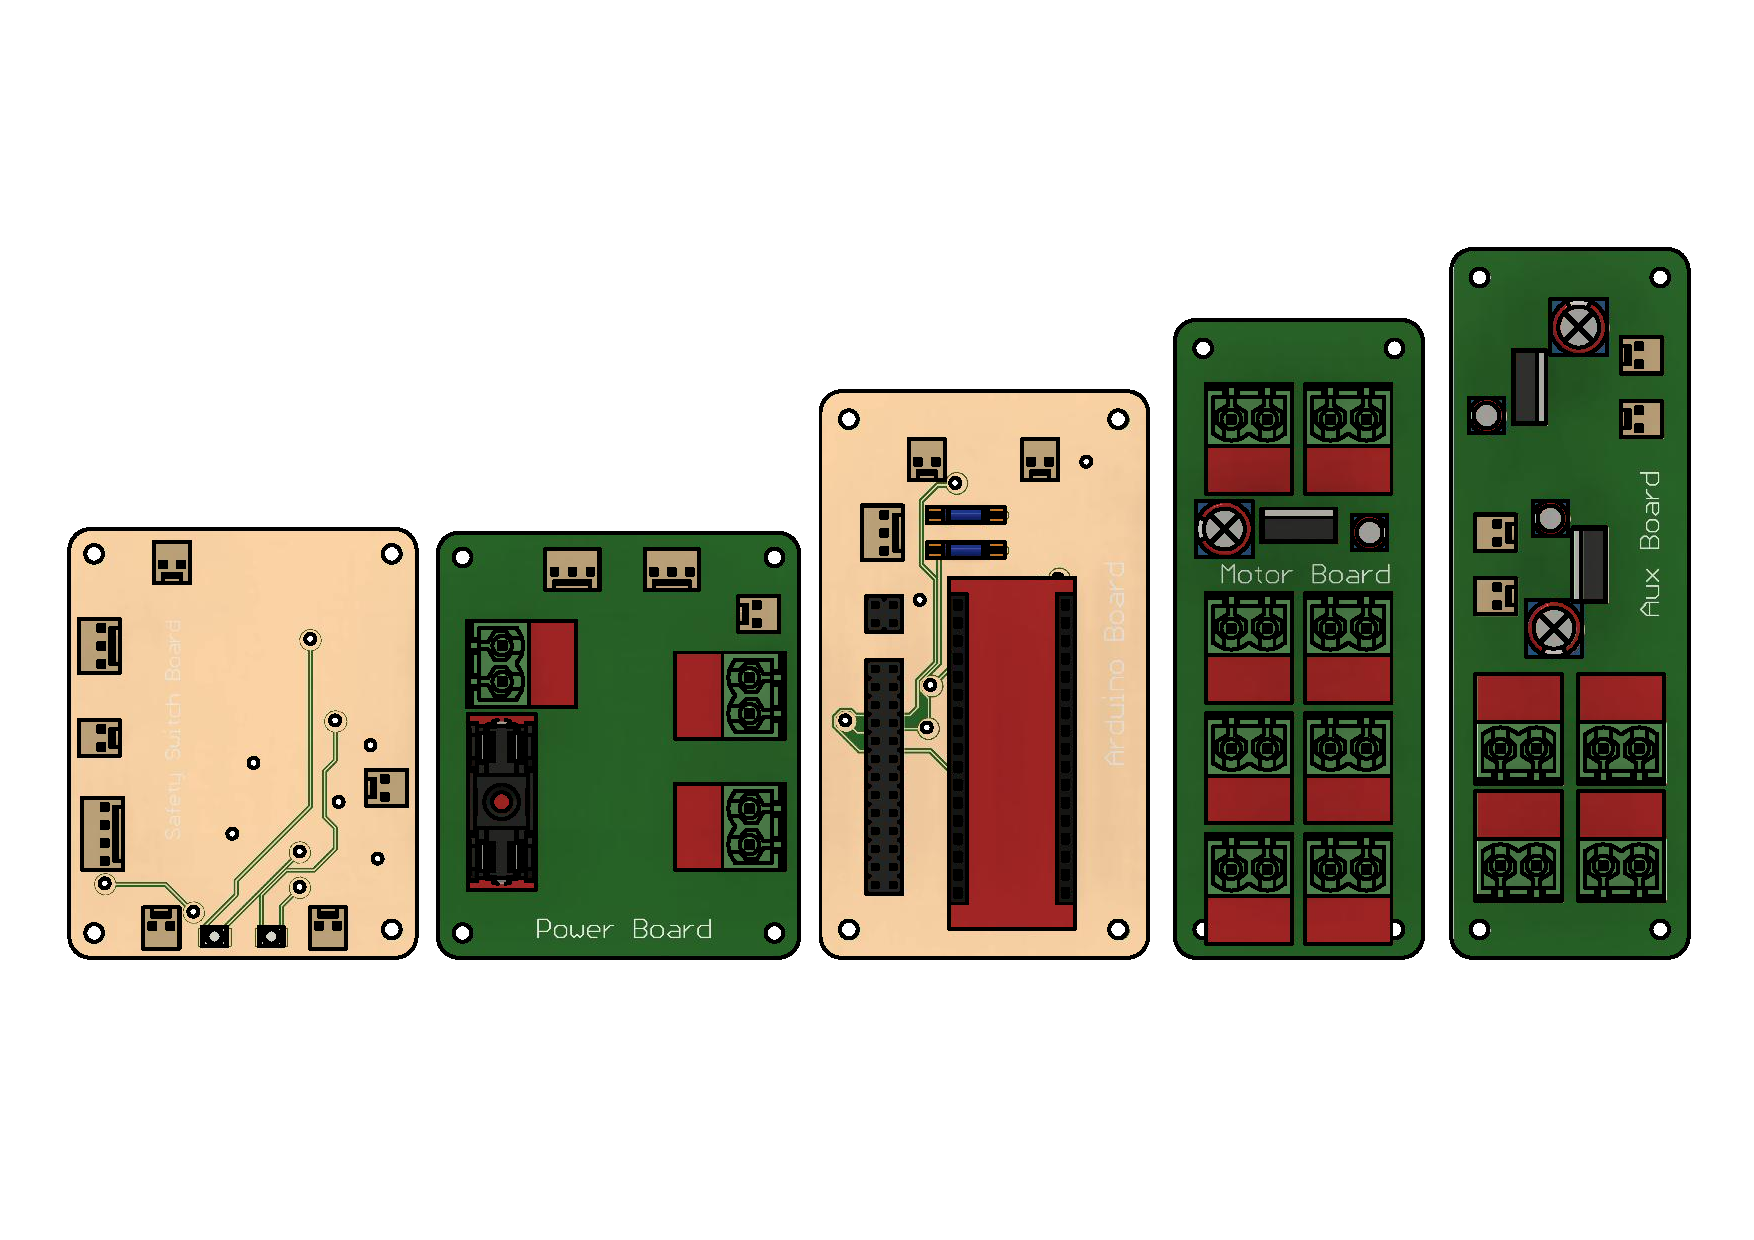
\includegraphics[width=1\textwidth]{Electronics/bulterpdb.pdf}
\caption{Top view of the boards in the PDB. From left to right: Safety Switch Board, Power Board, Arduino Board, Motor Board and Aux Board. The green areas are copper free areas and the red areas indicate connector clearance.}
\label{fig:butlerpdb}
\end{figure}

\subsubsection{Design}
The overall design to split the PDB into several boards has been chosen to simplify manufacturing and fault detection. This means that any issue is isolated to a single board and errors are more easily found. For complete specification of the boards see the manual. 

The Power Board is the main board that all power runs through. The power can be turned off with a main switch and the switching is done with MOSFETs\footnote{Metal–Oxide–Semiconductor Field-Effect Transistor}. The board has a fuse of 16 A installed to limit the maximum current. The Power Board has two power outputs controlled by the Safety Switch Board. The first output is the Motor output and it can supply a maximum of about 11 A. The second output is the auxiliary output and it can supply a maximum of about 10 A. 

The power is controlled from the Safety Switch Board. It controls the power to the outputs either from the main power switch or the safety switches. The board has four switches. The first switch is the main switch which controls the main power on or off. The second switch is a emergency switch which can disable the motors but having the control electronics enabled. The third switch is a magnetic switch that complements the emergency switch. A magnetic field need to be applied in the range of the magnetic switch to enable it. The fourth and last switch needs a "HIGH" digital signal in order to be enabled, this is controlled by the Arduino Board.
All switches are connected to an AND gate and needs to be "HIGH" for the Motor output to be enabled. In addition the Safety Switch Board as two LEDs, one green and one red, that indicate the status of the board. Green indicates that the board is on and all outputs are enabled and red indicates that at least one safety switch is not enabled so the motor output is disabled. Only one LED can be lit at the time.

The Motor Board is connected to the Power board and is basically an extension of the Power board. It has six outputs that use the battery voltage and two outputs that are regulated by a linear regulator at 12 V.

The Aux Board works by the same principle as the Motor board But is connected to the auxiliary output from the Power Board. It has four outputs that use the battery voltage and two 5 V and two 12 V linearly regulated outputs.

The Arduino board uses an Arduino Micro and communicates via I\textsuperscript{2}C bus connected to the Power Board were the voltage/current monitor is mounted. The Arduino Micro is programmed to monitor the voltage and current, this is to keep track of the voltage in order to determine when discharging of the battery should stop in order to protect the battery. The Arduino can then disable one of the safety switches which would disable the motors and the red LED will be lit. The Arduino board have been designed to be versatile with the pins from the Arduino Micro accessible for future functions.

\subsubsection{Future work}
The PDB have not been tested with the motors and the electronics, the only test that have been conducted is basic functionality. The PDB have not been wired on the Butler.

A battery have not been bought but the PDB was designed with the intention of using a LiFePO\textsubscript{4} battery from Biltema\footnote{\url{http://www.biltema.se/sv/}}. That battery have a voltage range of about 12.9 V to 14 V. If another battery with voltage below 12.9 V is going to be used, modifications need to be made to the PDB this is stated in the manual.

\subsection{System architecture - Ali Mokdad}
\begin{figure}[ht!]
\centering 
\includegraphics[width=1\textwidth]{Electronics/diagram.png}
\caption{Butler system architecture}
\label{fig:Butler system architecture}
\end{figure}

The system architecture of the Butler with the power requirements is shown in Figure~\ref{fig:Butler system architecture}. 
Table~\ref{table: The different motors for the Butler} lists brief explanation of each of the motors of the Butler.

\begin{table}[h!]
\centering
  \begin{tabular}{ | p{2cm}| p{9cm} |}
    \hline
    M1 arm  & Stepper motor for the first joint of the Butler arm   \\ \hline
    M2 arm  & Stepper motor for the second joint of the Butler arm   \\ \hline
    M3 arm  & Servo motor for rotating the hand. The feedback present in the diagram includes position, temperature, load, input voltage, etc.   \\ \hline
    M4 base & Dc motor with screw for moving all the arm up and down.\\ \hline
    M5 base & Stepper motor (same as M2 arm), for rotating the base of the Butler.\\
    \hline
  \end{tabular}
\caption{The different motors for the Butler}
\label{table: The different motors for the Butler}
\end{table}

\begin{table}[ht!]
\centering
  \begin{tabular}{ | p{2cm}| p{3cm} |}
    \hline
    M1 arm  & 14V, 0.4A    \\ \hline
    M2 arm  & 14V, 1.7A    \\ \hline
    M3 arm  & 12V, 2.2A    \\ \hline
    M4 base & 14V, 950 mA  \\ \hline
    M5 base & 14V, 1.7A    \\ \hline
    Cortex M4f & 5V        \\ \hline
    Jetson TX2 & 12 to 14V \\ \hline
  \end{tabular}
\caption{ Power requirements for the Butler}
\label{table: Power requirements for the Butler}
\end{table}

In the butler system: The PDB is responsible of providing power for the whole system. The Jetson TX2  is a full-featured development platform for visual computing, which constitutes the brain of the Butler; it communicates through a CAN bus with the Cortex M4f processor placed on a TM4C123G board which is an evaluation platform used for controlling the motors by sending the required PWM signals and serial communication (for the servo M3 hand) received from the Jetson TX2.
The LIDAR\cite{lidar} detection system which uses light from a laser to measure the distance to the object by illuminating that target with a pulsed laser light and send the data via USB communication to the Jetson TX2.
The Orbbec Astra Pro camera\cite{Camera} constitutes the eyes of the Butler, and the CHARLIE platform which is a different project platform will be used for this project. 